\documentclass[journal]{IEEEtran}
\usepackage{amssymb}
\usepackage{lineno}
\usepackage{fixltx2e}
\usepackage{hyperref}
\usepackage{enumitem}
\usepackage{amsmath}
\usepackage{graphicx}
\usepackage{listings}
\usepackage{tabularx}
\usepackage{xcolor}

\lstset{ %
	language=C,                % choose the language of the code
	basicstyle=\footnotesize,       % the size of the fonts that are used for the code
	numbers=none,                   % where to put the line-numbers
	numberstyle=\footnotesize,      % the size of the fonts that are used for the line-numbers
	stepnumber=1,                   % the step between two line-numbers. If it is 1 each line will be numbered
	backgroundcolor=\color{white},  % choose the background color. You must add \usepackage{color}
	showspaces=false,               % show spaces adding particular underscores
	showstringspaces=false,         % underline spaces within strings
	showtabs=false,                 % show tabs within strings adding particular underscores
	frame=single,           % adds a frame around the code
	tabsize=2,          % sets default tabsize to 2 spaces
	captionpos=b,           % sets the caption-position to bottom
	breaklines=true,        % sets automatic line breaking
	breakatwhitespace=false,    % sets if automatic breaks should only happen at whitespace
	escapeinside={\%*}{*)}          % if you want to add a comment within your code
}

\DeclareMathOperator*{\argmax}{arg\,max}

\begin{document}
	
\title{Comparing five common classification algorithms on facial and numeral images}

%% use optional labels to link authors explicitly to addresses:
%% \author[label1,label2]{<author name>}
%% \address[label1]{<address>}
%% \address[label2]{<address>}

\author{Christian~M.~Lillelund,~\IEEEmembership{201408354@post.au.dk,~School of Engineering, Aarhus University}% <-this % stops a space
\thanks{Manuscript received April 19, 2005; revised August 26, 2015.}}
\maketitle

%\address{School of Engineering, Aarhus University}

%\address{X}

\begin{abstract}
X
\end{abstract}

\begin{IEEEkeywords}
	IEEE, IEEEtran, journal, \LaTeX, paper, template.
\end{IEEEkeywords}

\section{Introduction}
For humans, it doesn't take much effort to tell the difference between a picture of a dog or a cat. A natural number or a letter. A happy person or a sad person. For computers, these sort of problems are notorious hard to solve and often require many computational resources. Machine learning and computer vision deals with these issues as they encompass a range of algorithms and classification techniques to produce a model or scheme that can tell images apart and recognize similarities. In this report we study the recognition and classification of a data set containing human faces and one featuring hand-written numbers by implementing and testing five commonly used techniques (Nearest class centroid classifier, nearest sub-class centroid, nearest neighbor and two perceptron variants) using MATLAB. We split the data in a training and a test set, then train our respective model or classifier and evaluate their ability to classify correctly on the testing set. A version using all the dimensions of the data and a principal component version will be applied. We use some visualization techniques to better communicate the data representation and tables to compare them. We start by going over the basic theory behind the classification schemes, then look at the data, briefly go over implementation details and then turn to results. At the end we review and argue which scheme would make the most sense to use with these two classification problems.

Initially, we split the ORL image data set, containing 400 40x30 pixel faces of 40 different persons, and the MNIST set containing 70.000 28x28 pixel hand-written numbers 0-9. The data is vectorized, so we use built-in MATLAB functions to construct the original pictures as such:

\begin{figure}[h]
	\centering
	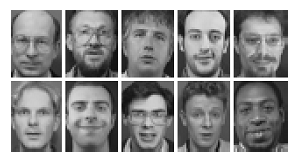
\includegraphics[width=0.7\linewidth]{orlfaces}
	\caption{Ten random images of faces from the ORL set.}
	\label{fig:orlfaces}
\end{figure}

\begin{figure}[h]
	\centering
	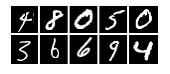
\includegraphics[width=0.7\linewidth]{mnistnumbers}
	\caption{Ten random images of numbers from the MNIST set.}
	\label{fig:mnistnumbers}
\end{figure}


\section{Theory}
This section will explain fundamental theory behind the dimensional reduction technique (PCA) and five schemes used in this report.

\subsection{Principal Component Analysis}

PCA is a procedure that transform a set of observations or samples in dimension $D$ to a lower dimension $D-n$ while still preserving a smaller number of variables explaining the main features $X_{1}, X_{2}, ..., X_{p}$ in the original set. This is particularly useful when dealing with high dimension data, as this can be computationally hard and challenging to visualize. With PCA, we compute principal components $d$ of $n$ original samples with $p$ features, where $d$ is the desired output dimensionality and each dimension is a linear combination of the $p$ features. In practice, we find eigenvectors of the covariance matrix of the original data set, sort them by highest eigenvalue score and use these as weights $W$ in computing a linear transformation $$y_{i} = W^T*x_{i}, i = 1, ..., N$$. The scattering of the transformed data is the scatter matrix, a function of $X$: $$S_{T} = \sum_{i=1}^{N} [W^T(x_{i}-\mu)][W^T(x_{i}-\mu)]^T$$. The weights $W$ can be found by applying eigenanalysis and taking the eigenvectors with the  highest score, more formally optimizing: \[ W* = \argmax_c Tr (W^TS_{T}) \] subject to $ W^TW=I$. We end with a data set containing fewer ($d < D$) dimensions.

\subsection{Nearest class centroid classifier}

The NCC classifier assigns labels $l_{i}$ to $N$ observations determined by which class $c_{k}$'s mean (centroid) the observation $x_{i}$ is closest to. We make the assumption that each class follow a normal distribution, as they are given equal importance in the classification algorithm. The mean class vector is given by: $$ \mu_{k} = \frac{1}{N_{k}} \sum_{i,li=k}^{} x_{i}, k = 1, ... K. $$

To classify any observation $x_{i}$ we find the smallest distance to any mean vector and assign the label of that vector to it, more formally: $$ d(x_{i},\mu_{k}) = ||x_{i}-\mu_{k}||^2_{2} $$

\subsection{Nearest subclass centroid classifier}

Similar to nearest class centroid, but each class $c_{k}$ now has subclasses $m$ that follow a normal distribution and has a mean vector $\mu_{km}$: $$ \mu_{km} = \frac{1}{N_{km}} \sum_{i,li=k, qi=m}^{} x_{i} $$ where $N_{km}$ denotes the number of observations in a given subclass and $x_{i}$ is a observation with a subclass label $qi$. Like NCC, the distance to the subclass mean is used to classify each observation: $$ d(x_{i},\mu_{km}) = ||x_{i}-\mu_{km}||^2_{2} $$

The number of subclasses is a hyper parameter for NSC and must be decided prior. Nearest subclass classifier is a compromise between nearest mean and nearest neighbor and combines the flexibility of nearest neighbor with the robustness of nearest mean, which we describer next. When the number of subclasses $m$ is equal to $N$ samples, we have the nearest neighbor classifier.

\subsection{Nearest neighbor classifier}

The nearest neighbor (NN) classifier is a simple algorithm where each sample is assigned to the class of its closest neighbor, or the most common class among its $k$ nearest neighbors in the k-NN variant. Pure NN is when $k=1$, but often $k>1$ where a majority vote takes place. The algorithm uses euclidean distance between a test sample $x_{i}$ with class $c_{k}$ and a training one $y_{i}$: $$ d(x_{i},y_{i}) = ||x_{i}-y_{i}||^2_{2} $$

\subsection{Perceptron learning with backpropagation}

A perceptron is a supervised algorithm of binary classifiers, that classify whether or not an input sample $x_{i}$ belong to class $c_{k}$. It uses the linear discriminant function $f(x) = w^T*x + w_{0}$, where $w$ are weights, $x\varepsilon$ $\mathbb{R^D}$ a feature vector and $w_{0}$ the bias. $w$ represent the orientation of the discriminant hyperplane, and $w_{0}$ a offset from the origin. Given weights $w$, sample $x_{i}$ and classes $c_{1}$ and $c_{2}$, the function splits the feature space into these two classes. If $g(w,x_{i}) > 0$, $x_{i}$ belongs to $c_{1}$ and if $g(w,x_{i}) < 0$, $x_{i}$ belongs to $c_{1}$. If $g(w,x_{i}) = 0$, it can be classified to either class. The resulting scalar is the distance of $x_{i}$ to the hyperplane. The function is used in our perceptron to follow, where we define a binary label $l_{i}$ for each sample to express the criterion function: $$ f(w^*,x_{i}) = l_{i} g(w,x_{i}) = l_{i} w^{*T} x_{i} \geq 0, i = 1, ..., N $$

All samples are correctly classified, if $f(w_{*}, x_{i}) \geq 0$. To produce such result, we need to optimize weights $w_{*}$ by the perceptron criterion function for $w_{*}$, where ${\jmath}_{p}(w_{*}) = 0$ would be a solution for $w_{*}$: $$ {\jmath}_{p}(w) = \sum_{x_{i} \varepsilon \chi}^{} -f(w,x_{i}) = \sum_{x_{i} \varepsilon \chi}^{} -l_{i} w^T x_{i} $$

To optimize ${\jmath}_{p}(w)$, we use the gradient at $w$ and follow it to update $w$, where $\eta$ is the rate of change (learning rate) and expresses how fast it converges, and $\varepsilon$ express a vector set of mislabeled samples:

$$ w(t+1) = w(t) - \eta(t) \nabla{\jmath}_{p} = w(t) + \eta(t) \sum_{x_{i} \varepsilon \chi}^{} l_{i} x_{i} $$

At each learning iteration, the weights $w(t)$ are "punished" by the sum of misclassified samples scaled, leading to convergence as the result of criterion function ${\jmath}_{p}$ will be higher. This is known as backpropagation. The algorithm to come will elaborate on this.

\subsection{Perceptron learning with MSE}

As an alternative to backpropagation, one can apply least-mean square regression to obtain the perceptron weights $W$. Here we use a criterion function ${\jmath}_{LSE}$ that involves all of the samples, not just the misclassified ones. Previously we made the inner products of $f(X) = W^T*X$ positive, now we look to find a solution to $W^T X = t_{i}, i = 1, ..., N$, where $t_{i}$ are arbitrarily set positive constants. This is written as $X^T*w = b$ in matrix form. If X is nonsingular, we could write $W = X^-1 b$ and have a formal solution, but this is often not the case, however by obtaining the pseudo-inverse of $X$ one can find a solution for the weights: $$ X^\dagger = (X^tX)^{-1}X^T $$

Examining the criterion function, we look to minimize: $$ {\jmath}_{LSE} = ||W^T X - B||^2_{F} $$

By setting the derivative of this to zero with respect to $W$, we get: $$ \nabla{\jmath}_{LSE} = 0 => 2XX^W = 2XB^T $$

Hence: $$ W = (XX^T)^{-1} XB^T = W^\dagger B^T $$

If W is square and nonsingular, the pseudo-inverse is simply the regular inverse. Also it holds at $X^\dagger X = I$, but $X X^\dagger \neq I$, though a MSE always exists, hence $W = X^\dagger b$ is an MSE solution to $X^\dagger w = b$.

\section{Implementation}

The implementation uses MATLAB to design and run the different schemes on the training data and evaluating on the test data. For understanding purposes, this section will briefly lay out the algorithms described in theory as pseudo-code how we implemented them.

\subsection{PCA} 

The algorithm centers the data, then simply calculates eigenvectors from the variance matrix, sort them after highest eigenvalue and uses the $n$ vector as principal components in representing the data. Listing \ref{lst:pca} shows this.

\begin{minipage}[t]{0.95\linewidth}
	\begin{lstlisting}[caption=Implementation of PCA., label={lst:pca}]
	pca_reduce(trainData, nDimensions) {
		trainData = trainData - mean(trainData) for rows in trainData
		eigVectors, eigValues = eig(cov(trainData))
		eigVectors = sort(eigVectors, 'descending')
		pc = eigVectors[from 1 to nDimensions]*trainData
	}
	\end{lstlisting}
\end{minipage}

\subsection{NCC} 

Simply calculate a mean vector for $c_{k}$ classes by summing the samples that belong te class and dividing that with the number of $N$ samples in a given class, as expressed in listing \ref{lst:ncc}.

\begin{minipage}[H]{0.95\linewidth}
	\begin{lstlisting}[caption=Implementation of NCC., label={lst:ncc}]
	train_ncc(trainData, trainLbls, nClasses) {
		mu = zero vector by size of trainData*nClasses
		n = zero vector by size of 1*nClasses
		index = 1;
		
		for (i = 1; i <= nClasses;i++) {
			n(i) = sum(num of classes i in trainLbls)
			mu(i) = sum(each traning sample from index to n(i))/n(i)		
			index = index+n(i)
		}
	}
	\end{lstlisting}
\end{minipage}

\subsection{NSC} 

We make an initial k-means clustering of the training data for $k=m$ subclasses as hyper parameter and use the resulting centroids to construct a new centroid matrix for each subclass $m$ spanning $c_{k}$*$m$. Listing \ref{lst:nsc} shows this.

\begin{minipage}[H]{0.95\linewidth}
	\begin{lstlisting}[caption=Implementation of NSC., label={lst:nsc}]
	train_nsc(trainData, trainLbls, nC, nSubClasses) {
	centroids = zero vector by size of trainData*(nClasses*nSubClasses)
	n = zero vector by size of 1*nClasses
	index = 1;
	centroidIdx = vector to keep index of centroids
	
	for (i = 1; i <= nClasses;i++) {
		n(i) = sum(num of classes i in trainLbls)
		[idx,clst] = kmeans(trainData for index+n(i), nSubClasses)
		centroids()
		index = index+n(i)
	}
		
		
	mu(i) = sum(each traning sample from index to n(i))/n(i)		
	index = index+n(i)
	}
	}
	\end{lstlisting}
\end{minipage}







%\end{frontmatter}

%% The Appendices part is started with the command \appendix;
%% appendix sections are then done as normal sections
%% \appendix


%% \section{}
%% \label{}

%% References
%%
%% Following citation commands can be used in the body text:
%% Usage of \cite is as follows:
%%   \cite{key}          ==>>  [#]
%%   \cite[chap. 2]{key} ==>>  [#, chap. 2]
%%   \citet{key}         ==>>  Author [#]

%% References with bibTeX database:

\bibliographystyle{model1-num-names}
\bibliography{literature.bib}

%% Authors are advised to submit their bibtex database files. They are
%% requested to list a bibtex style file in the manuscript if they do
%% not want to use model1-num-names.bst.

%% References without bibTeX database:

% \begin{thebibliography}{00}

%% \bibitem must have the following form:
%%   \bibitem{key}...
%%

% \bibitem{}

% \end{thebibliography}
 

\end{document}